\section{Part 1.1: Sequential FedAvg}\label{sec:p11}
\subsection{Implementation and aggregation}
Let $n_k$ denote client $k$'s \emph{training} count and $S_t$ the sampled set at round $t$. Each selected client receives an identical copy of $w_t$, initializes a fresh SGD optimizer, and executes $E$ complete local epochs, including the final short minibatch. If its final parameters are $w_{t+1}^{(k)}$, the synchronous server computes
\begin{equation}
 w_{t+1}=\sum_{k\in S_t}\frac{n_k}{\sum_{j\in S_t}n_j}w_{t+1}^{(k)}.\label{eq:fedavg}
\end{equation}
Weights use only selected clients' training counts. Uniform sampling without replacement selects exactly 2, 5, or 10 of the 100 eligible clients for $C=0.02,0.05,0.10$. Aggregation waits for all valid updates; invalid rounds are rejected. The implementation uses PyTorch and NumPy without a specialized federated-learning package.

\subsection{Question 1: overall and five-client class distributions}
Global class counts range from 56 examples for class 45 to 1,837 for class 24, a 32.8-fold difference (\cref{fig:overall}). The five clients in \cref{fig:five,tab:five} represent extremes of training size and observed-class count, plus a typical client. Client 86 minimizes squared standardized distance to the median size, diversity, and entropy profile among the remaining clients. Selection uses data characteristics, not model performance.

\begin{figure}[htbp]
\centering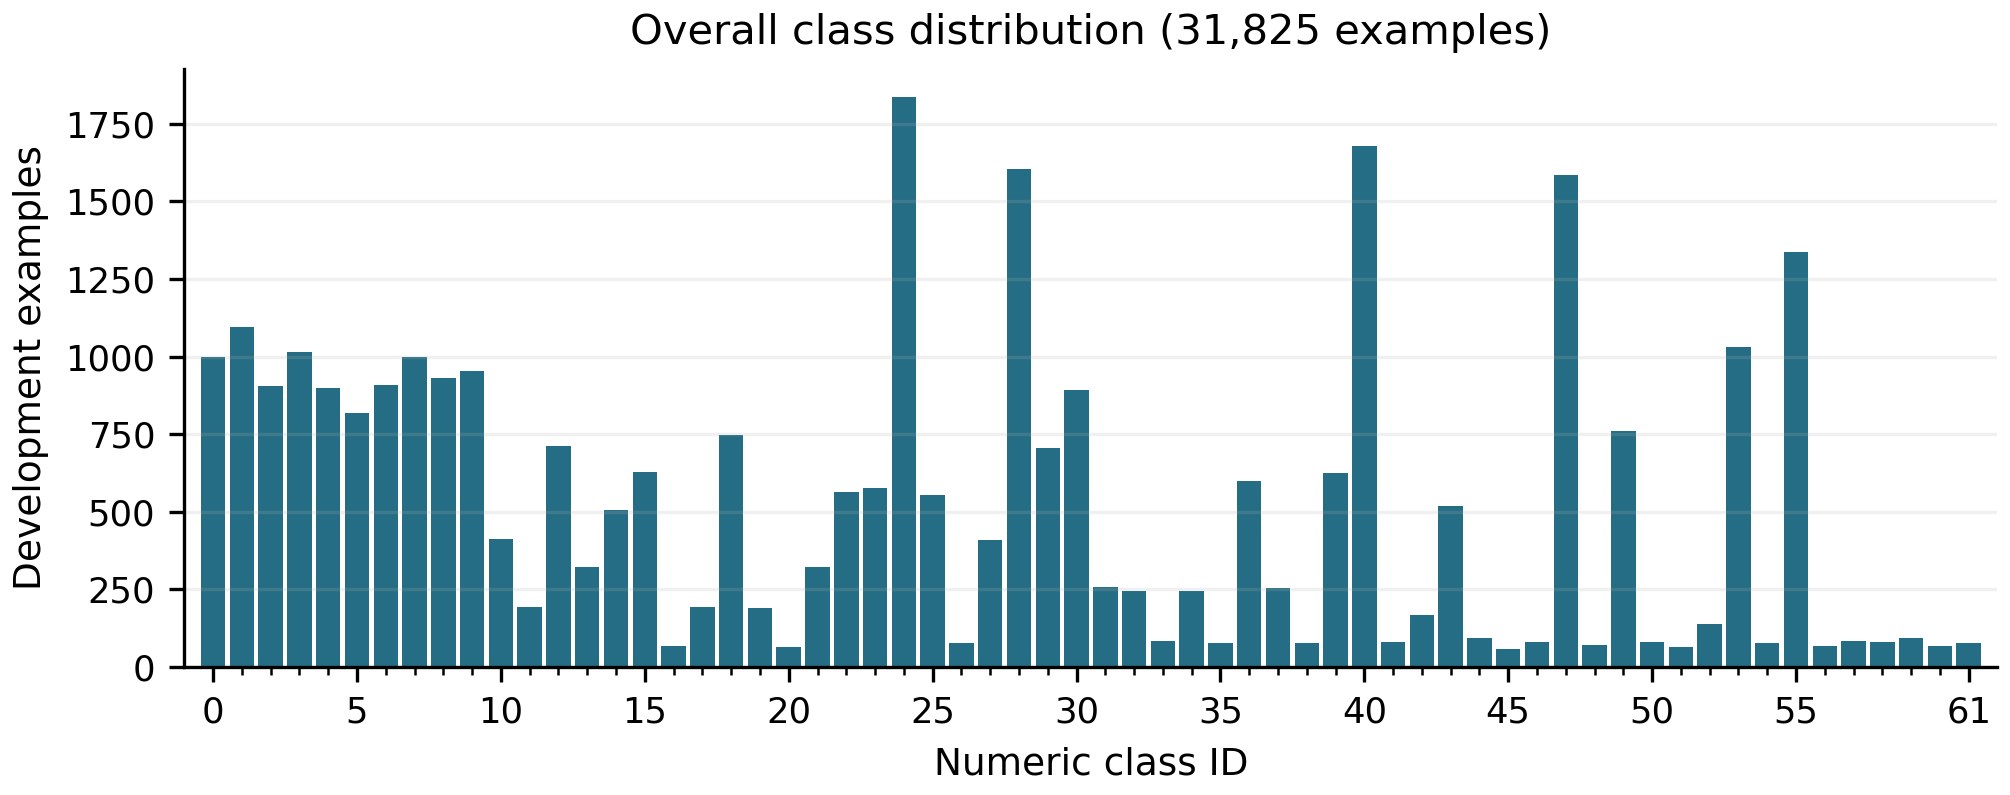
\includegraphics[width=\linewidth]{figures/part1_1/overall_class_distribution.png}
\caption{Counts for all 62 numeric labels in the complete 31,825-example development pool. Peaks and rare classes establish global imbalance; no undocumented character mapping is inferred.}\label{fig:overall}
\end{figure}
\begin{table}[htbp]
\centering
\caption{Five clients selected using training-set characteristics. Entropy is $H_k=-\sum_c p_{kc}\log_2p_{kc}$ over locally observed training labels.}\label{tab:five}
\begin{tabular}{rlrrr}
\toprule
ID & Selection reason & Train / validation & Classes & $H_k$ (bits)\\
\midrule
67 & Largest training set & 314 / 79 & 54 & 5.084\\
25 & Smallest training set & 94 / 24 & 38 & 4.802\\
16 & Most observed classes & 300 / 75 & 57 & 5.221\\
36 & Fewest observed classes & 182 / 46 & 37 & 4.964\\
86 & Median profile & 260 / 65 & 51 & 5.115\\
\bottomrule
\end{tabular}
\end{table}
\begin{figure}[htbp]
\centering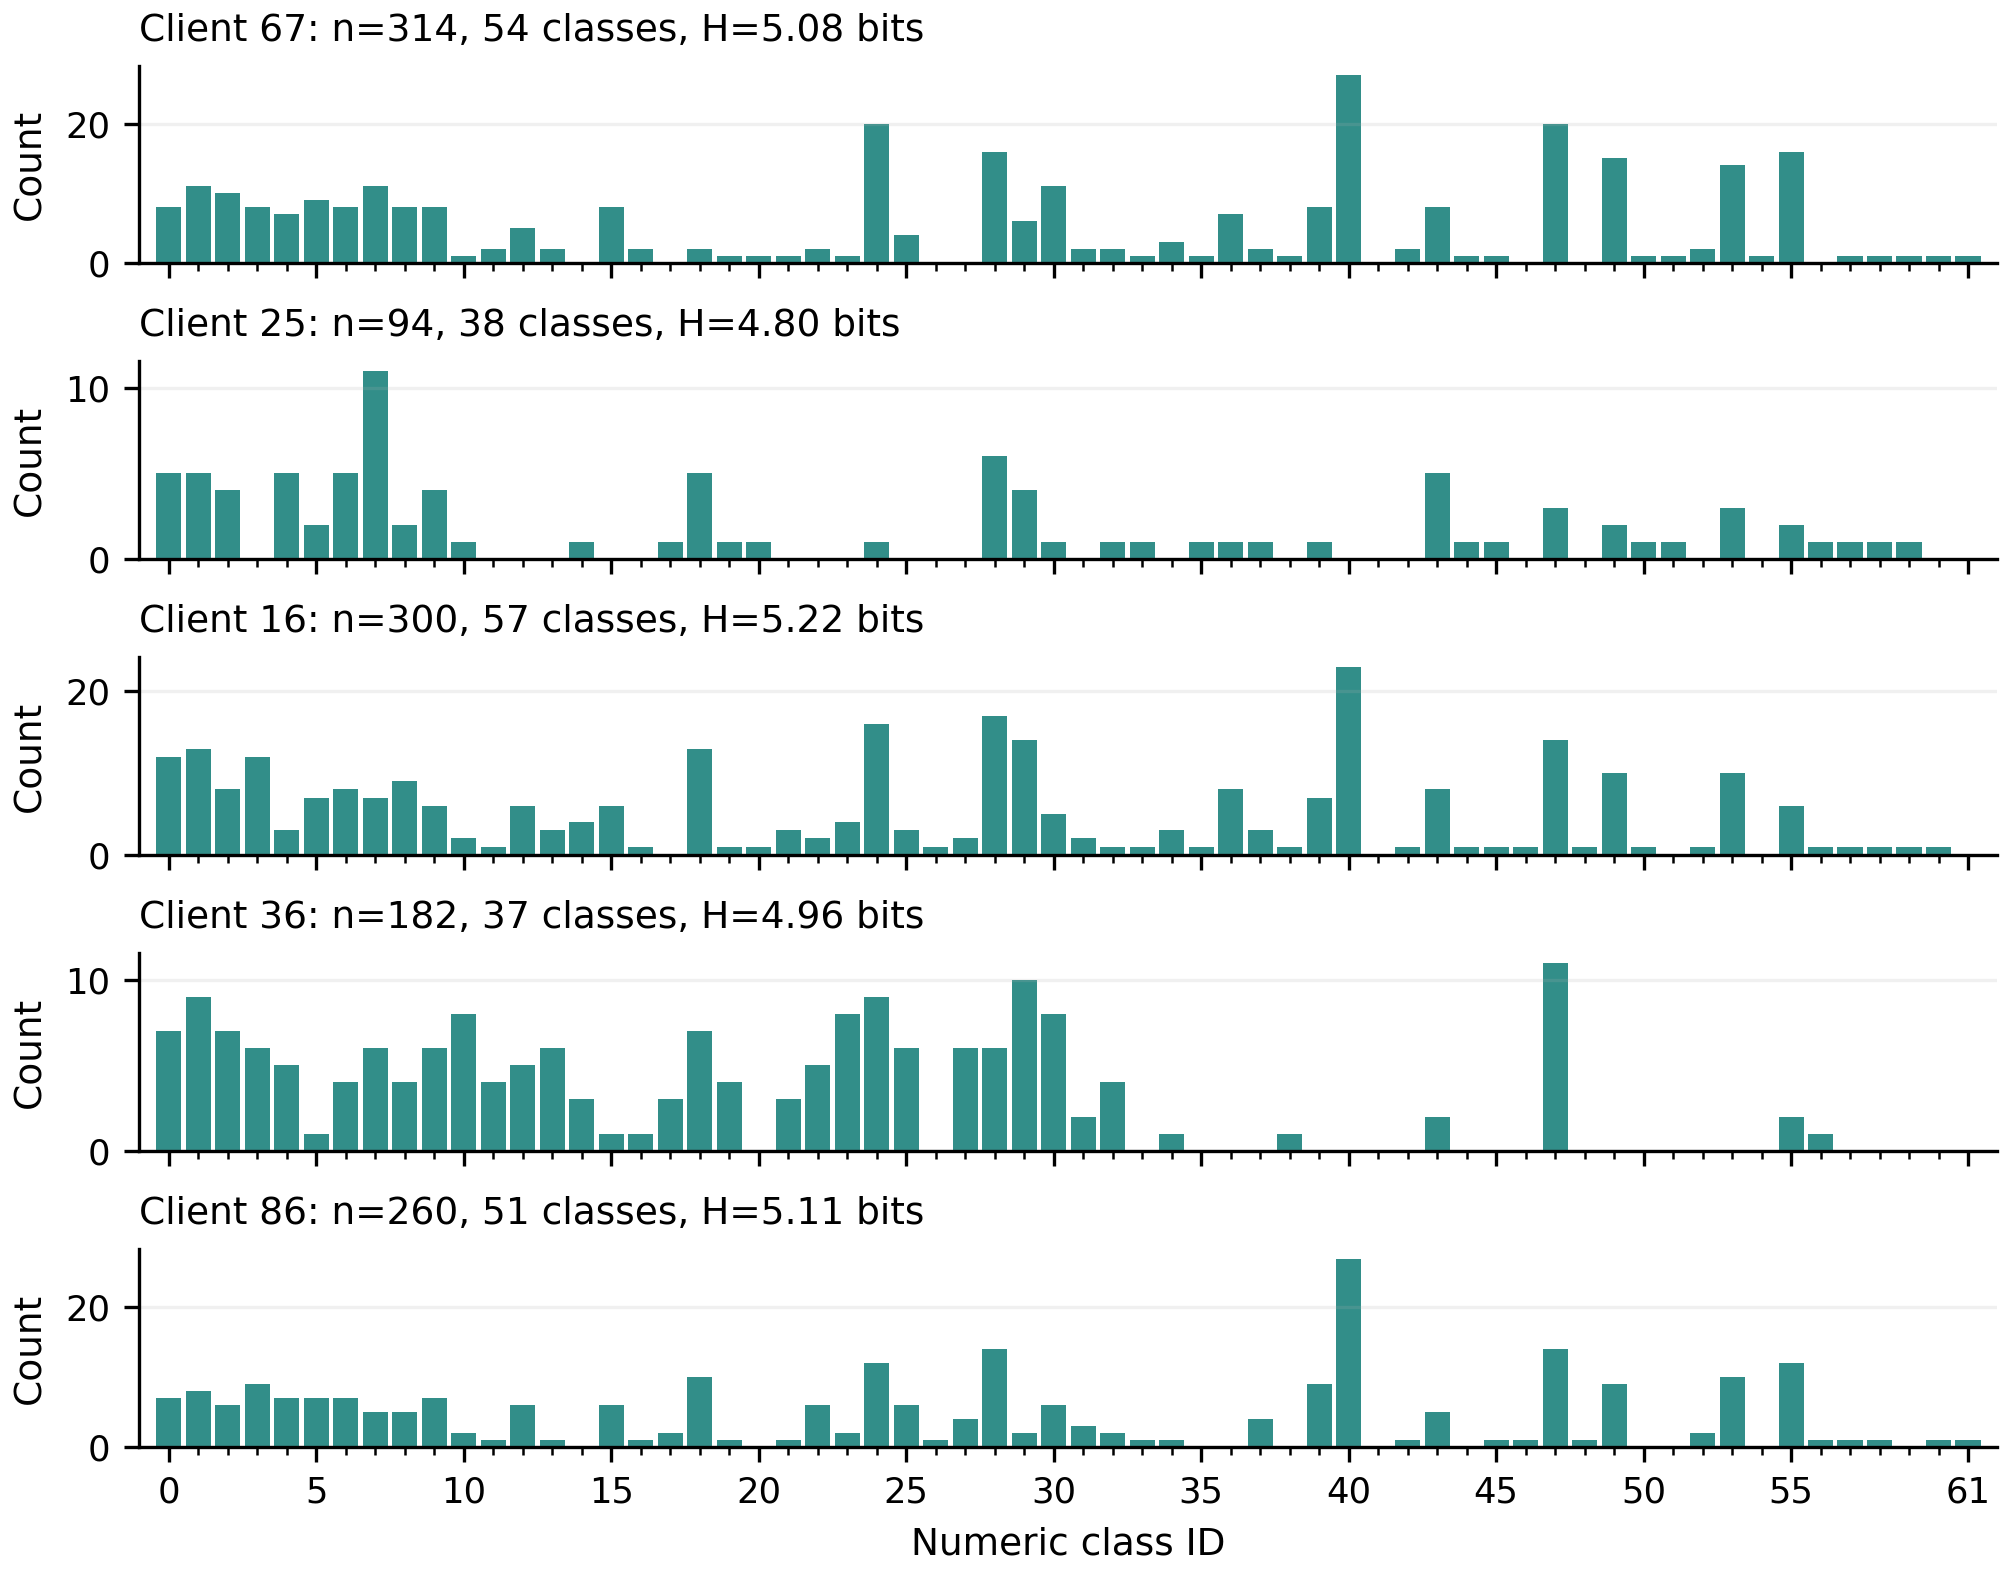
\includegraphics[width=\linewidth]{figures/part1_1/five_client_distributions.png}
\caption{Training-label counts for five systematically chosen clients. The shared numeric-label axis exposes missing classes and differing local proportions. These panels use training subsets, whereas \cref{fig:overall} uses the full development pool.}\label{fig:five}
\end{figure}

Training-label entropy averages 5.111 bits across clients (range 4.682--5.272). The differing proportions, missing labels, and unequal counts characterize empirical heterogeneity; entropy captures label mix rather than handwriting style. The controlled partition experiment below tests how stronger label segregation affects learning.

\subsection{Questions 2--4: baseline convergence and hyperparameter comparison}
The baseline uses $C=0.10$, $E=1$, learning rate 0.3, batch size 32, seed 2026, and 80 rounds. A preceding six-run, 12-round pilot compared learning rates 0.01, 0.1, and 0.3 at $E=1,3$ with $C=0.10$. The mean final validation accuracies over the two epoch settings were 6.86\%, 28.33\%, and 46.69\%, respectively. The largest mean selected the shared rate 0.3 before the main grid; test data were not used.

At the baseline, training/validation accuracy rises from 3.19\%/3.03\% to 67.02\%/65.29\%. Training cross-entropy falls from 4.126150 to 1.246401 and validation cross-entropy from 4.126700 to 1.328689 (\cref{fig:baseline}).
\begin{figure}[htbp]
\centering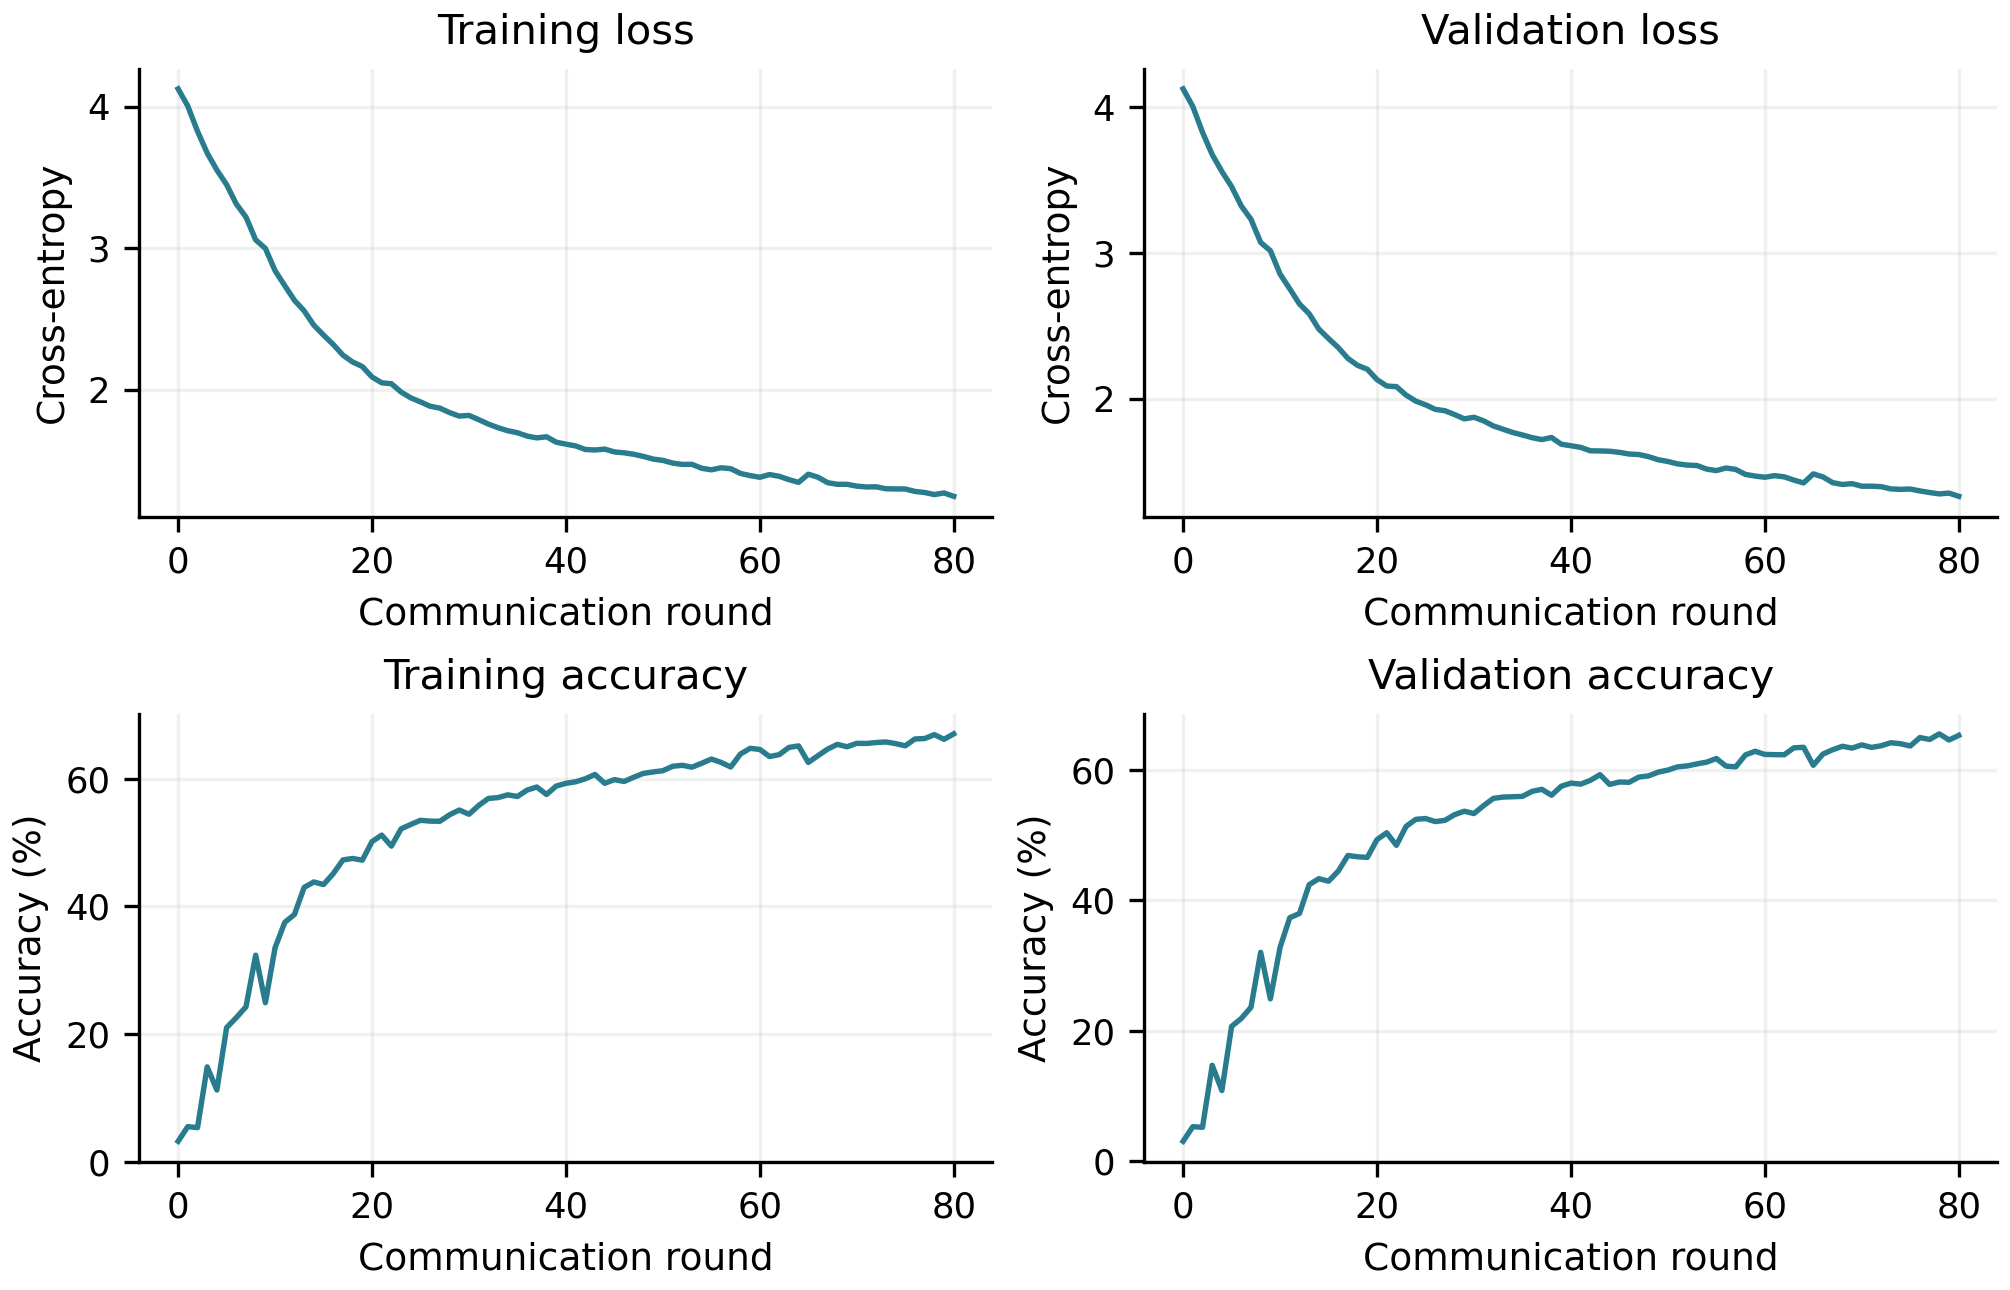
\includegraphics[width=\linewidth]{figures/part1_1/baseline_convergence.png}
\caption{Required full-pool training and validation loss/accuracy curves for sequential FedAvg, $C=0.10$, $E=1$, seed 2026. Round zero is the initialized model. Each later point evaluates the updated global model, not an average of selected clients' local models.}\label{fig:baseline}
\end{figure}

\begin{table}[htbp]
\centering
\caption{Main 80-round comparison, seed 2026, learning rate 0.3 and batch size 32. Accuracies are percentages. Best validation and final validation are distinct.}\label{tab:grid}
\begin{tabular}{rrrrrrr}
\toprule
$C$ & $E$ & Final train & Final val. & Best val. (round) & Client-epochs & Exposures\\
\midrule
0.02 & 1 & 60.83 & 59.03 & 61.28 (78) & 160 & 40,949\\
0.02 & 3 & 69.99 & 67.64 & 69.39 (77) & 480 & 122,847\\
0.05 & 1 & 66.40 & 64.66 & 64.66 (80) & 400 & 102,161\\
0.05 & 3 & 74.85 & 72.59 & 72.98 (78) & 1,200 & 306,483\\
0.10 & 1 & 67.02 & 65.29 & 65.52 (78) & 800 & 203,782\\
0.10 & 3 & 75.32 & 73.00 & 73.00 (80) & 2,400 & 611,346\\
\bottomrule
\end{tabular}
\end{table}
\begin{figure}[htbp]
\centering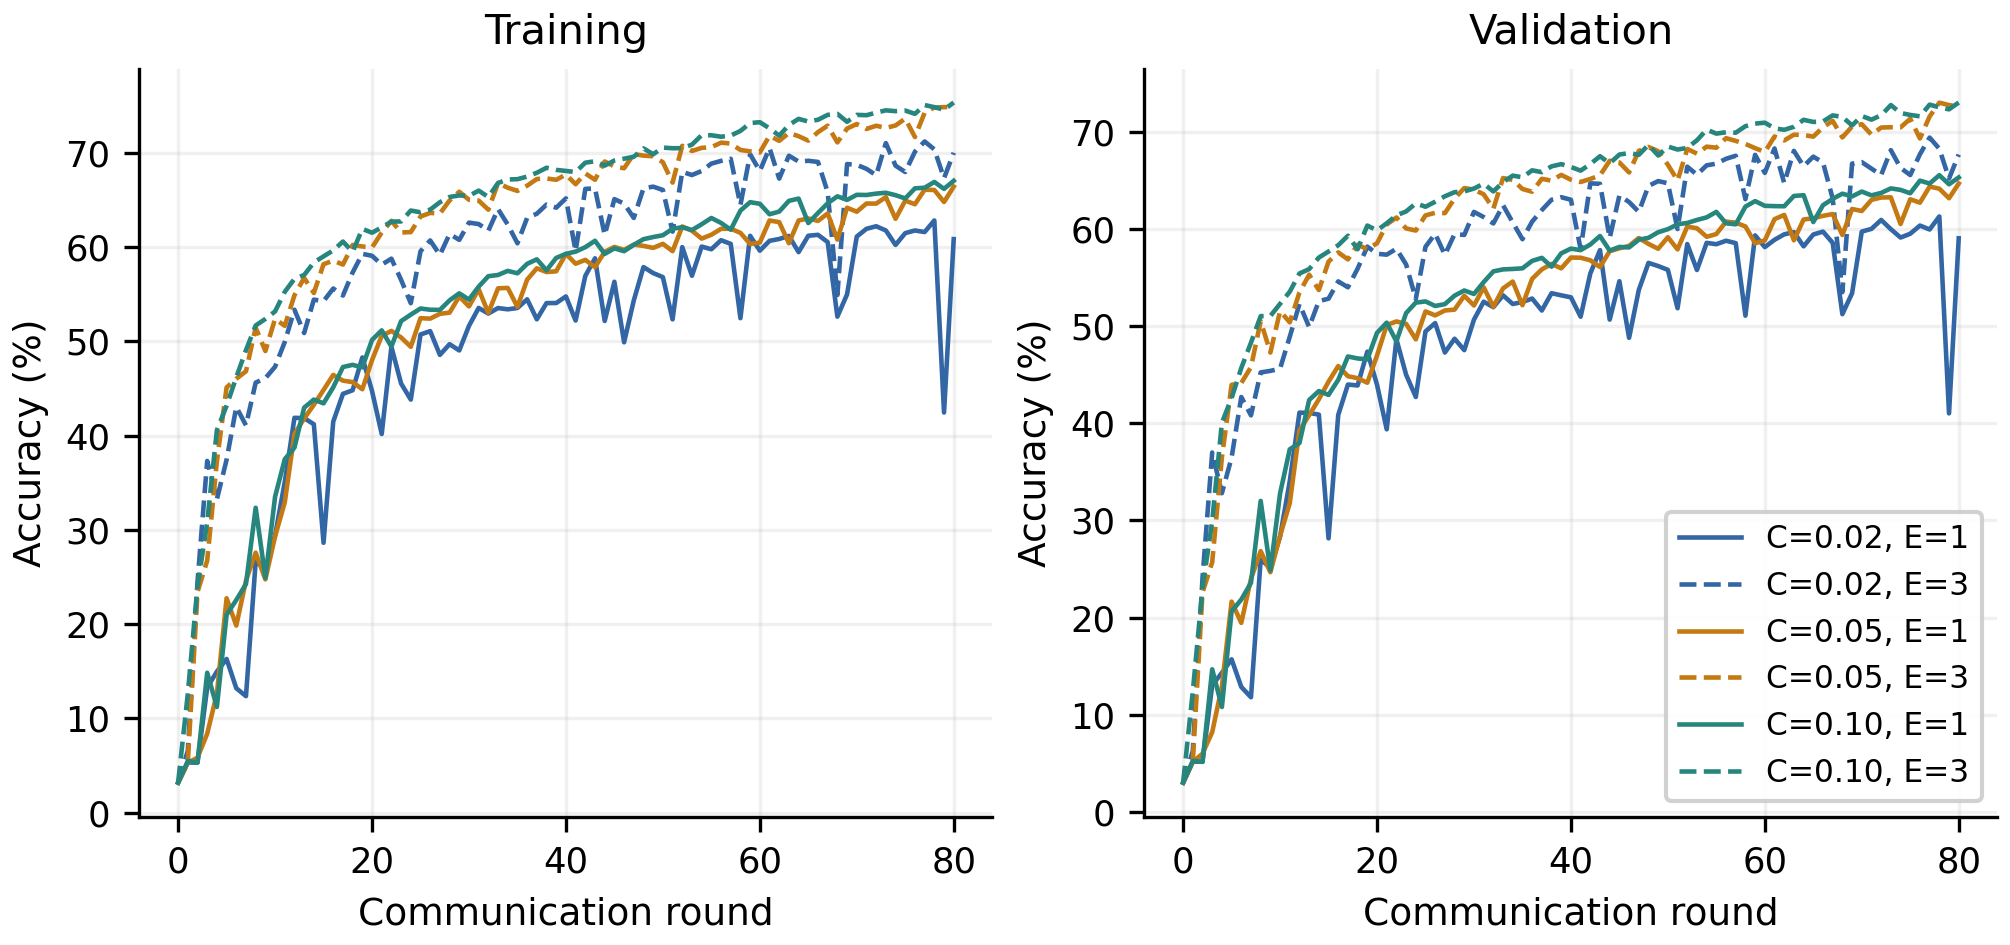
\includegraphics[width=\linewidth]{figures/part1_1/hyperparameter_accuracy.png}
\caption{Training and validation accuracy for the six $(C,E)$ settings. Colors encode client fraction and line style encodes local epochs. The shared round budget is a communication-round comparison, not a matched-computation experiment.}\label{fig:grid}
\end{figure}

Increasing $E$ from 1 to 3 improves final validation accuracy by 8.62, 7.93, and 7.71 percentage points at $C=0.02,0.05,0.10$. These paired-schedule comparisons also triple sample exposures. Larger $C$ generally improves final accuracy and stability while increasing per-round computation. The 80-round grid spans 160--2,400 client-epochs; \cref{tab:grid} reports actual exposures and \cref{fig:cost} shows the corresponding computation tradeoff.

For $C=0.02,E=1$, the largest one-round validation decline is 20.26 points and the last-ten-round SD is 6.05 points; at $C=0.10,E=3$, these decrease to 1.39 and 0.60 points. These trajectory statistics combine trend and sampling fluctuations, rather than independent-run uncertainty. Larger local budgets help here, but stronger heterogeneity can induce client drift \citep{courseFL}.

\subsection{Question 5: validation selection and held-out evaluation}
The two leading primary-seed configurations were repeated at seeds 2027 and 2028. Mean best validation accuracy was $71.94\%\pm0.99\pp$ for $C=0.05,E=3$ and $72.77\%\pm0.23\pp$ for $C=0.10,E=3$; mean final accuracy was $71.52\%\pm1.14\pp$ and $72.40\%\pm0.57\pp$, respectively (sample SD). Maximizing mean best validation selected $C=0.10,E=3$, after which the highest-validation seed/checkpoint was seed 2026, round 80.

The selected model correctly classifies 2,684/3,621 held-out examples: \textbf{74.12\% test accuracy}, with cross-entropy 0.986716. This is the validation-selected seed-2026 result. At fixed round 80, the selected configuration ($C=0.10$, $E=3$, learning rate 0.3, batch size 32) achieves 74.12\%, 72.88\%, and 73.13\% at seeds 2026--2028: a mean of $73.38\%\pm0.66\pp$ (sample SD). These evaluations use the same 3,621 test examples and are supported by Part 2's exactly matched zero-noise trajectories (\cref{sec:p2validation,tab:allnoise}); they describe seed variability rather than independent test datasets.

The primary-seed best-validation advantage over $C=0.05,E=3$ is only $100/6407=0.0156$ points, or one example, so that contrast alone is not evidence of significant superiority. Test evaluation followed the frozen validation selection.

\subsection{Scientific Validation and Edge Cases}\label{sec:p11validation}
\subsubsection{Mathematical correctness: unequal-count aggregation and the SGD identity}
To verify aggregation independently of model accuracy, we compared the implemented update with a manually computed mean of three float32 vectors weighted by counts $[1,3,6]$. The expected vector is $[-0.5,2.8,5.4]$. Maximum error is $2.3841858\times10^{-7}$, below the $10^{-6}$ tolerance, confirming the unequal-count arithmetic.

A second test connects the implementation to a known optimization identity. With all clients participating, one full-batch local SGD step gives
\begin{align}
w_{t+1}^{(k)}&=w_t-\eta\nabla F_k(w_t),\nonumber\\
\sum_k\frac{n_k}{N}w_{t+1}^{(k)}
&=w_t-\eta\sum_k\frac{n_k}{N}\nabla F_k(w_t)
=w_t-\eta\nabla F(w_t),\label{eq:sgdidentity}
\end{align}
Here $F_k$ is a local mean loss and $F$ the pooled mean. With 17 synthetic examples split 2/5/10, the actual 62-output MLP, learning rate 0.03, and one full local batch per client, FedAvg differs from centralized SGD by at most $7.4505806\times10^{-9}$ (tolerance $3\times10^{-7}$). This tests loss normalization, optimization, and aggregation together. The identity applies to this one-step special case; multiple local steps evaluate gradients at different client weights.

\subsubsection{Stochastic correctness: participation and repeatability}
Sampling was checked with 10,000 draws per fraction, verifying subset size, uniqueness, and exact replay of a seeded stream. Under independent rounds, a client's marginal participation count has mean $TC$ and SD $\sqrt{TC(1-C)}$.
\begin{table}[htbp]
\centering
\caption{Sampling diagnostic over 10,000 rounds per fraction. Every subset has the required unique-client count and the same-seed streams match exactly.}\label{tab:sampling}
\begin{tabular}{rrrrr}
\toprule
$C$ & Expected count & Binomial SD & Observed min--max & Maximum $|z|$\\
\midrule
0.02 & 200 & 14.000 & 166--230 & 2.429\\
0.05 & 500 & 21.794 & 432--574 & 3.395\\
0.10 & 1,000 & 30.000 & 924--1,069 & 2.533\\
\bottomrule
\end{tabular}
\end{table}
All participation deviations lie below the five-SD threshold (\cref{tab:sampling}), consistent with the intended marginal sampling probabilities. Exact replay and across-seed learning stability address different questions; \cref{fig:seeds} shows the latter for the two leading settings.

\subsubsection{Positive and negative learning controls}
The positive control tests whether SGD learns a known spatial signal and responds to learning rate. Twenty synthetic clients provide 960 training and 320 validation examples for a balanced binary task, using the unchanged 62-output model. With matched initialization and selections over 25 rounds, learning rate 0.1 reaches 100\% validation accuracy and reduces training loss from 4.051352 to 0.00257871; rate 0.0001 reaches only 1.25\%. The result exceeds the criteria of $>90\%$ accuracy, halving the loss, and a $>20$-point advantage.

The negative control permutes training labels within each client while preserving counts, label frequencies, validation data, initialization, selections, and optimizer settings. After 40 rounds at $C=0.10,E=3$, correct labels yield 66.36\% validation accuracy versus 7.65\% with randomized labels, a 58.72-point gap against a 15-point criterion. Learning thus depends strongly on image--label correspondence. The residual accuracy is compatible with imbalance and preserved local label frequencies; $1/62$ is not an appropriate universal reference for this control.

\subsubsection{Controlled heterogeneity intervention}
To isolate the effect of partition structure, we reassigned the 25,418 training examples to the original client-size vector by either random permutation or label sorting. Validation remained unchanged. Both 40-round runs used the same schedule, $C=0.10,E=3$, and 306,447 example exposures, removing size and computation differences from the comparison.

Label segregation reduces mean entropy from 5.1836 to 0.3780 bits and final validation accuracy from 69.88\% to 27.81\%, a 42.06-point gap (\cref{fig:controls}). This controlled response is consistent with stronger client drift under multi-step SGD. Only this intervention reallocates data; all main experiments retain the original writers.

\begin{figure}[htbp]
\centering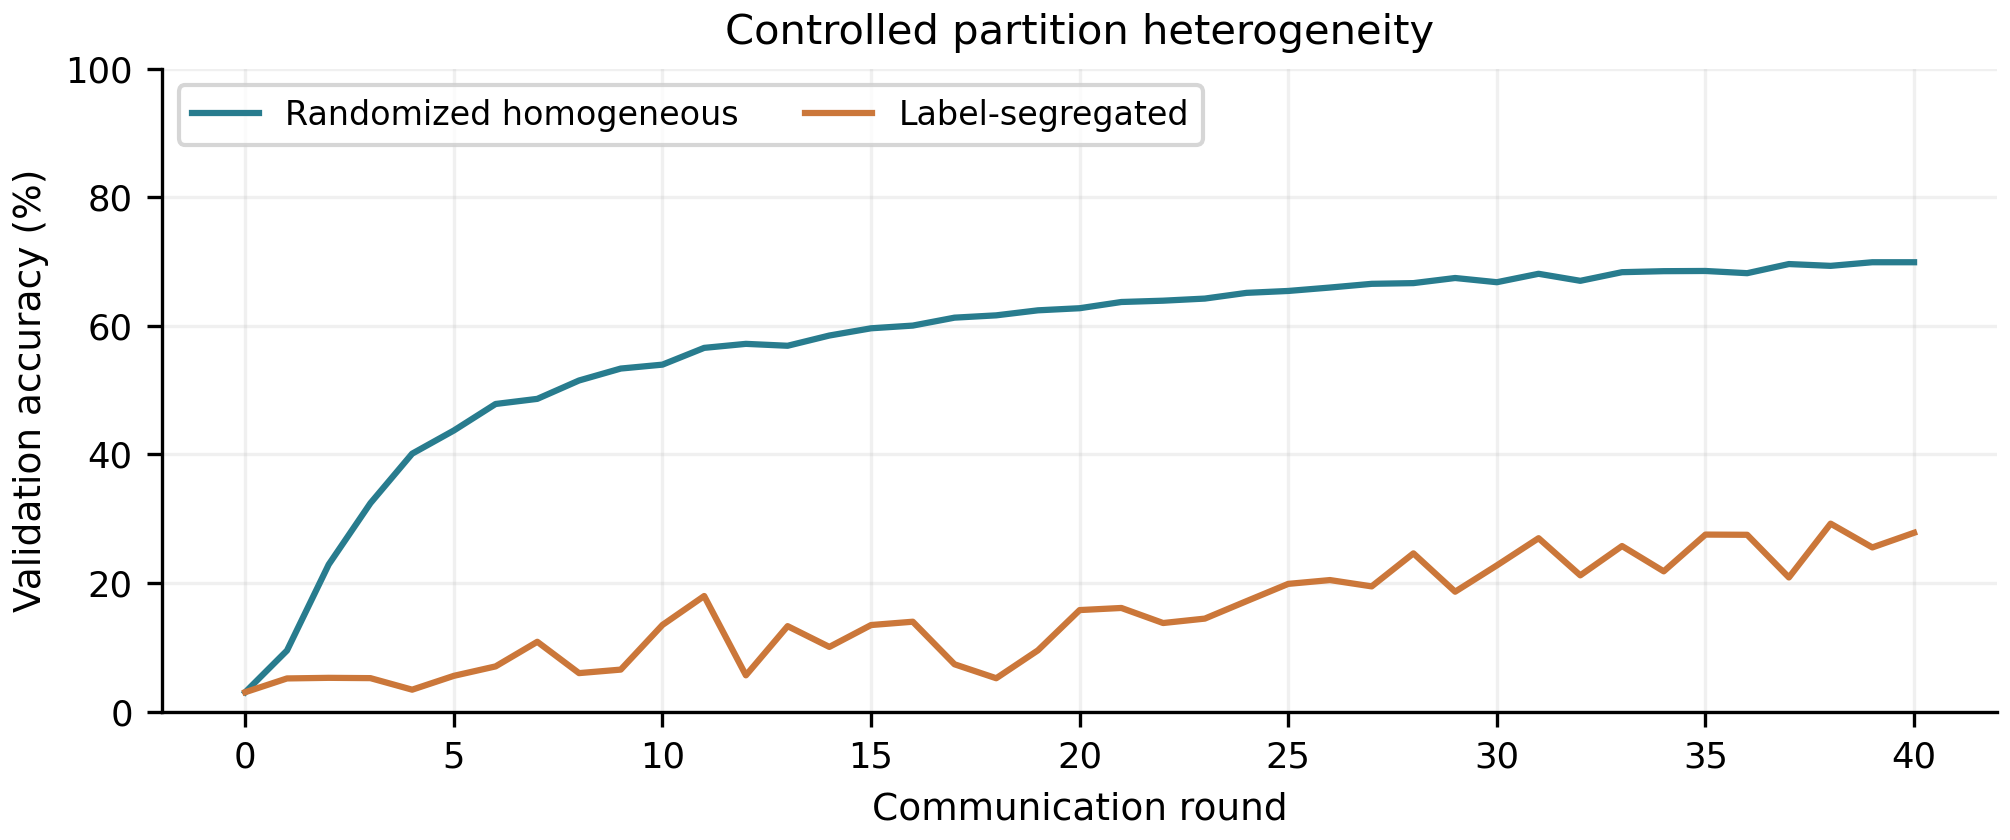
\includegraphics[width=\linewidth]{figures/part1_1/scientific_controls.png}
\caption{Validation accuracy under randomized and label-segregated training partitions. Both preserve client sizes, 306,447 sample exposures, and clean validation data over 40 rounds; $C=0.10$, $E=3$.}\label{fig:controls}
\end{figure}

\subsubsection{Non-standard visualization: who benefits from participation?}
\Cref{fig:benefit} relates participation to local validation improvement for the $C=0.10,E=1$, seed-2026 baseline. Counts range from 2 to 13 against an expectation of 8. Correlations of improvement with participation, training size, and entropy are $-0.0937$, $0.2895$, and $-0.0680$, respectively.

\begin{figure}[htbp]
\centering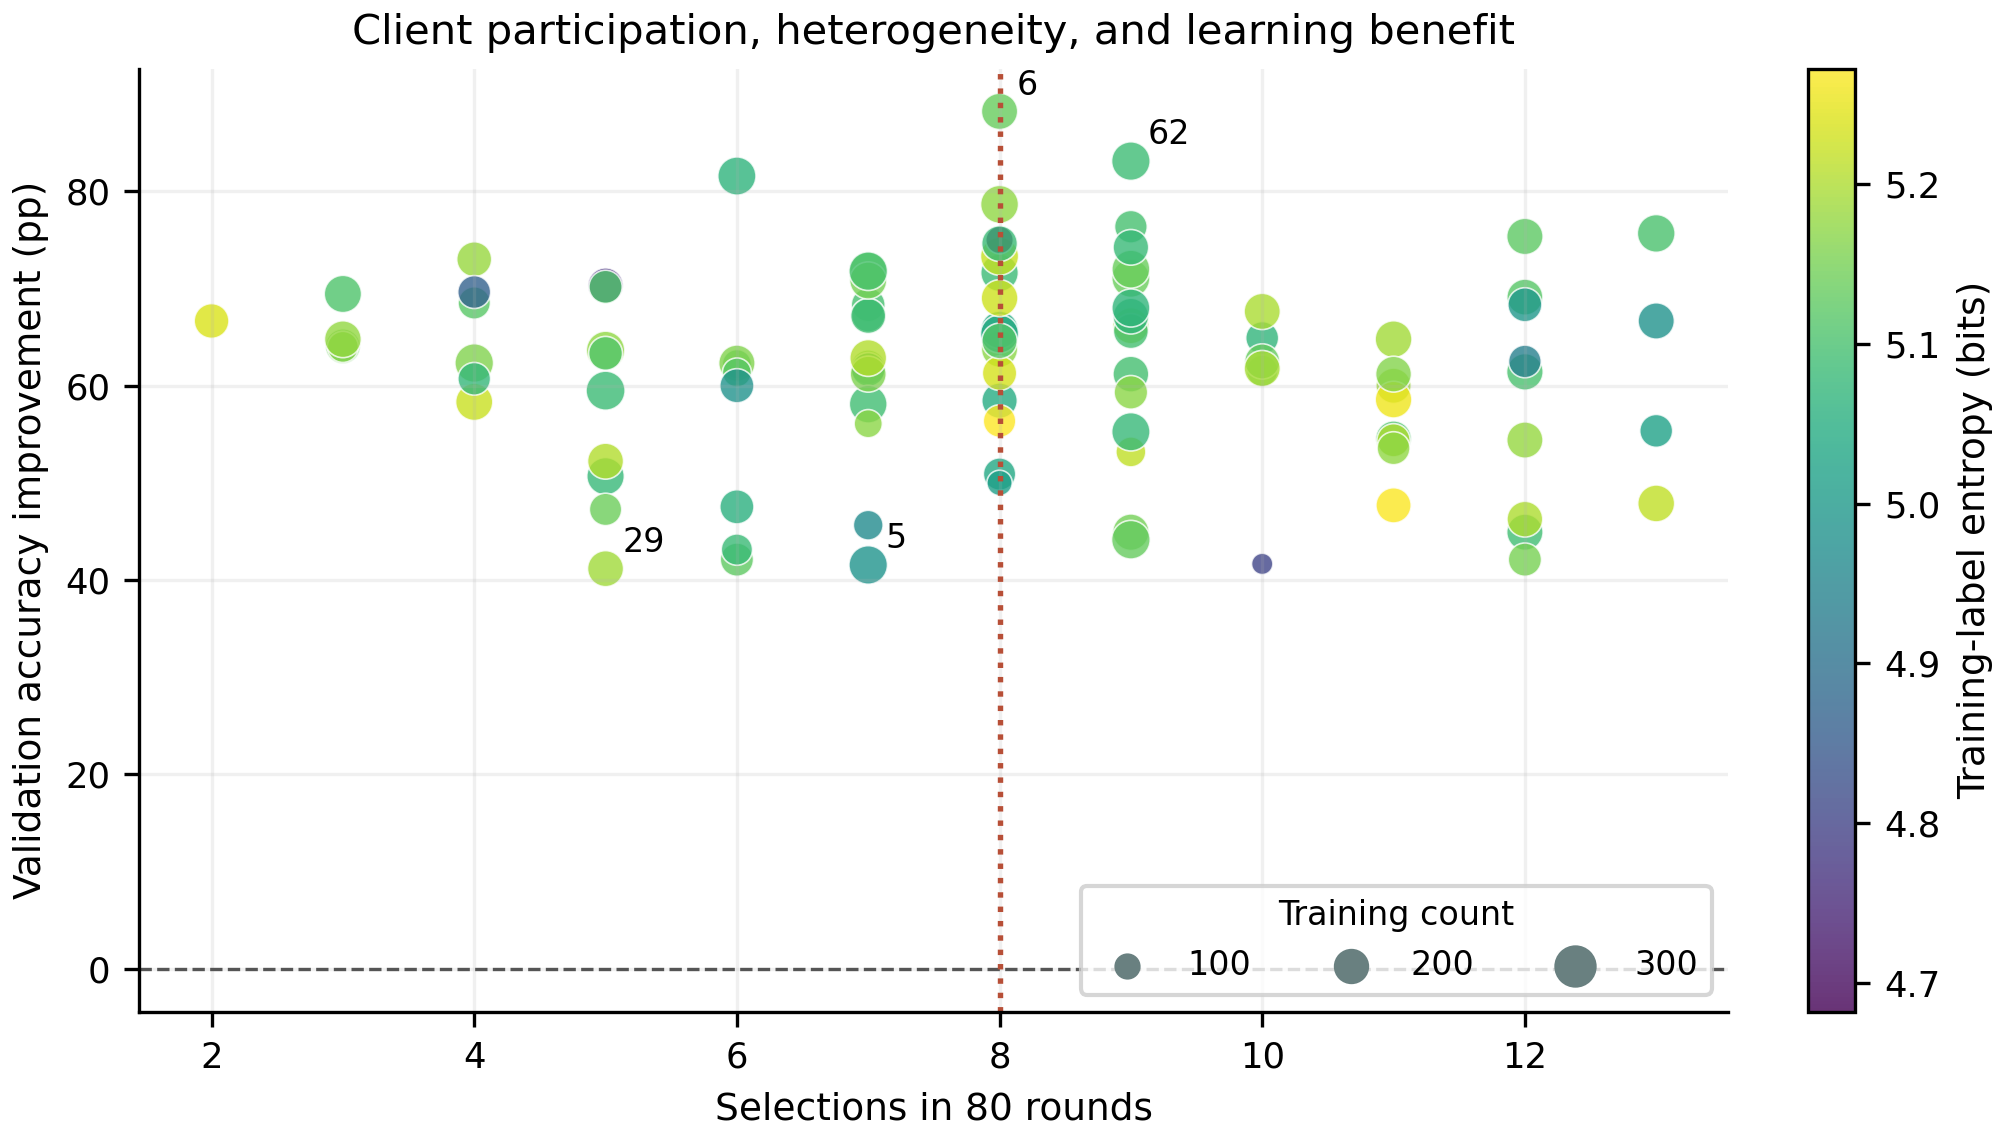
\includegraphics[width=\linewidth]{figures/part1_1/participation_heterogeneity_benefit.png}
\caption{Client participation and validation improvement from round 0 to 80, $C=0.10$, $E=1$, seed 2026. Point area represents training count and color represents label entropy. The reference line marks expected participation $80(0.10)=8$.}\label{fig:benefit}
\end{figure}

Bottom/top training-size quartiles improve by 57.87/65.26 points on average; client 29 improves by 41.18 points and client 6 by 88.24. Benefit is not monotone in participation, because every client receives a global model shaped by others. These exploratory associations describe unequal benefits rather than causal effects of size or participation.

\subsubsection{Robustness, invalid inputs, and restart behavior}
\begin{table}[htbp]
\centering
\caption{Edge-case handling and quantitative checks for Part 1.1. The 13-test suite completed with zero failures or errors.}\label{tab:p11edges}
\begin{tabularx}{\linewidth}{p{0.22\linewidth}YY}
\toprule
Case & Policy / design & Evidence and scope\\
\midrule
Empty and tiny clients & $n=0$ ineligible; $n=1$ training-only; $n\ge2$ has disjoint nonempty subsets. & Coverage/disjointness fixtures include 0, 1, 2, 3, 4, 5, 118, 393. No actual supplied client is empty.\\
Missing classes & Retain all 62 outputs; no fabricated examples. & Singleton class-zero training and empty local validation are checked.\\
Unequal counts & Use positive integer training counts. & A 1:99,999 count fixture averages values 0 and 10 to 9.9999 (five-decimal check).\\
Weighted metrics & Sum counts and losses across clients. & Zero-logit model on sizes 1 and 9 gives accuracy 0.1 and loss $\log62$, not unweighted accuracy 0.5.\\
Invalid updates & Reject NaN/Inf, empty update sets, duplicate IDs, bad counts, incompatible tensors. & Explicit exception assertions; invalid local losses are separately tested.\\
Broadcast / restart & Clone broadcast; create fresh optimizer; commit complete rounds atomically. & Repeated local updates preserve input digest; a three-round stop/resume fixture matches final state digest and selections.\\
Extreme learning rate & Record deterioration or reject non-finite arithmetic. & At $\eta=10^6$, synthetic loss reaches 155,043.09; this run stays finite and does \emph{not} trigger the non-finite guard.\\
\bottomrule
\end{tabularx}
\end{table}

The excessive-rate case in \cref{tab:p11edges} distinguishes finite arithmetic from useful learning: loss remains finite but becomes extremely large. Separate injected-NaN tests verify explicit rejection, while stop/resume tests verify exact recovery at committed round boundaries.



